\documentclass[a4paper,12pt]{article}

\usepackage[left=1in, right=1in, top=0.5in, bottom=1in]{geometry}
\usepackage[latin2]{inputenc} 
\usepackage{amsmath}
\usepackage{graphicx} 
\usepackage[T1]{fontenc} 
\usepackage{color}
\usepackage{amssymb} 
\usepackage{times}
\usepackage{subfig}

\newcommand{\lhood}{\ensuremath{\mathcal{L}}}
\newcommand{\truth}{\ensuremath{\mathcal{D}}}
\newcommand{\test}{\ensuremath{\mathcal{T}}}
\newcommand{\model}{\ensuremath{\mathcal{M}}}
\newcommand{\optmodel}{\ensuremath{\mathcal{M}^*}}

\DeclareMathOperator*{\argmin}{arg\,min}
\DeclareMathOperator*{\argmax}{arg\,max}

% Some useful macros

\definecolor{Cgreen}{rgb}{0,0.6,0}
\definecolor{Cblue}{rgb}{0,0.39,0.61}

\newcounter{ohNoteCounter} \newcommand{\ohnote}[1]{{\scriptsize
    \color{Cgreen}
    $\clubsuit$~\refstepcounter{ohNoteCounter}\textsf{[OH]$_{\arabic{ohNoteCounter}}$:{#1}}}}

\newcounter{jpNoteCounter} \newcommand{\jpnote}[1]{{\scriptsize
    \color{Cblue} $\blacksquare$
    \refstepcounter{jpNoteCounter}\textsf{[JP]$_{\arabic{jpNoteCounter}}$:{#1}}}}

\IfFileExists{.notes_disabled}{ \renewcommand{\jpnote}[1]{}
  \renewcommand{\ohnote}[1]{} }

\title { \normalsize Graphical Markov Models \\ Winter 2011 \\
 \vspace{10mm} {\bf Identifying License Plates Ids with Hidden Markov
    Models } }
\author{\normalsize James Pritts and Ondrej Hrstka }
\date{ \small January 2012 }

\begin{document}
\maketitle

\pagestyle{empty} 
\section*{1. DRAFT}
\section{Problem Statement}
The problem is to report the unique identifying string of characters,
called the \emph{vehicle-id}, of a license plate.  Provided are images
of license plates that have been segmented and ortho-rectified. A
subset of these images each have the following corresponding
annotations: a top and bottom boundary that delimits the
\emph{vehicle-id} within the segmented license plate, a bounding box
of each character and white-space interval that comprises the
\emph{vehicle-id}, and a character label for each bounding box that
contains a character.  We assume that the font of all characters
across license plates is identical, and we refer to a particular
character of the font set as a glyph.

\section{Preliminaries}
Let $I\colon \mathbb{Z}^2_+ \to \mathbb{R}$ be a function that maps a
point $\mathbf{u} = (i,j)$ to a real value $x_{ij}$, such that $I$
gives the raw intensity value at each point in the image.  Denote
$\mathbf{x}_i$ and $\mathbf{x}_j$ as the row and column of pixels in
the image at row $i$ and column $j$ respectively.

To condense the notation for probability distributions, we denote
$p_{x_{ij} \mid s_j}(x_{ij} \mid s_j)$ by writing $p(x_{ij} \mid
s_j)$; in other words, the arguments of $p$ will uniquely select the
proper density function for evaluation.

\section{Model Definition}
We model a \emph{vehicle-id} by a Hidden Markov Model (\textbf{HMM}).
The characters of the \emph{vehicle-id} are assumed to come from the
same font set, so any image of a particular character can be mapped to
the same glyph.  The left-to-right sequence of consecutive columns
from the segmented license plate are the \emph{observations}.

The set of \emph{hidden states} $\mathbf{K}$ are the column indexes of
all the glyphs in the font set and an added state $w$ that represents
white-space. An example sequence of hidden states $S \in \mathbf{K}^n$
is
\[S =
\left(\,\dots,\text{w},\text{A}_1,\text{A}_2,\ldots,\text{A}_{m},\text{w},\text{w},\text{w},\text{T}_1,\text{T}_2,\ldots\,\right).\]

The \emph{emission probabilities} are the probabilities of observing
pixel intensities given their corresponding glyph column, or,
equivalently, given their \emph{hidden states}. We make the
simplifying assumption that probabilities of observing intensities in
a column $\mathbf{x}_j$ are pairwise independent \[p(\mathbf{x}_j \mid
s_j) = \prod_{i=1}^np(x_{ij} \mid s_j).\] The probability of observing
pixel intensity $x_{ij}$ of a glyph column $s_j$ is modeled as a
two-class gaussian mixture, where the first class $c=f$ contains
foreground pixels, and the second class $c=b$ contains background
pixels,
\begin{align*}
  p(x_{ij} \mid s_j) &= p(x_{ij},c=f \mid s_j)+p(x_{ij},c=b \mid s_j)\\
  &= p(x_{ij}\mid c=f,s_j)p(c=f \mid s_j)+p(x_{ij} \mid c=b,s_j)p(c=b \mid s_j) \\
  &= p(x_{ij}\mid c=f)p(c=f \mid s_j)+p(x_{ij} \mid c=b)p(c=b \mid s_j) \\
  &= \mathcal{N}(\sigma_1,\mu_1)\gamma_{is_j}+\mathcal{N}(\sigma_2,\mu_2)(1-\gamma_{is_j}).
\end{align*}
The model for \emph{emissions probabilities} assumes that the
foreground and background distributions are position independent,
while the mixture parameter depends on the row position of the glyph
column $s_j$.

\begin{figure}[htp]
\centering
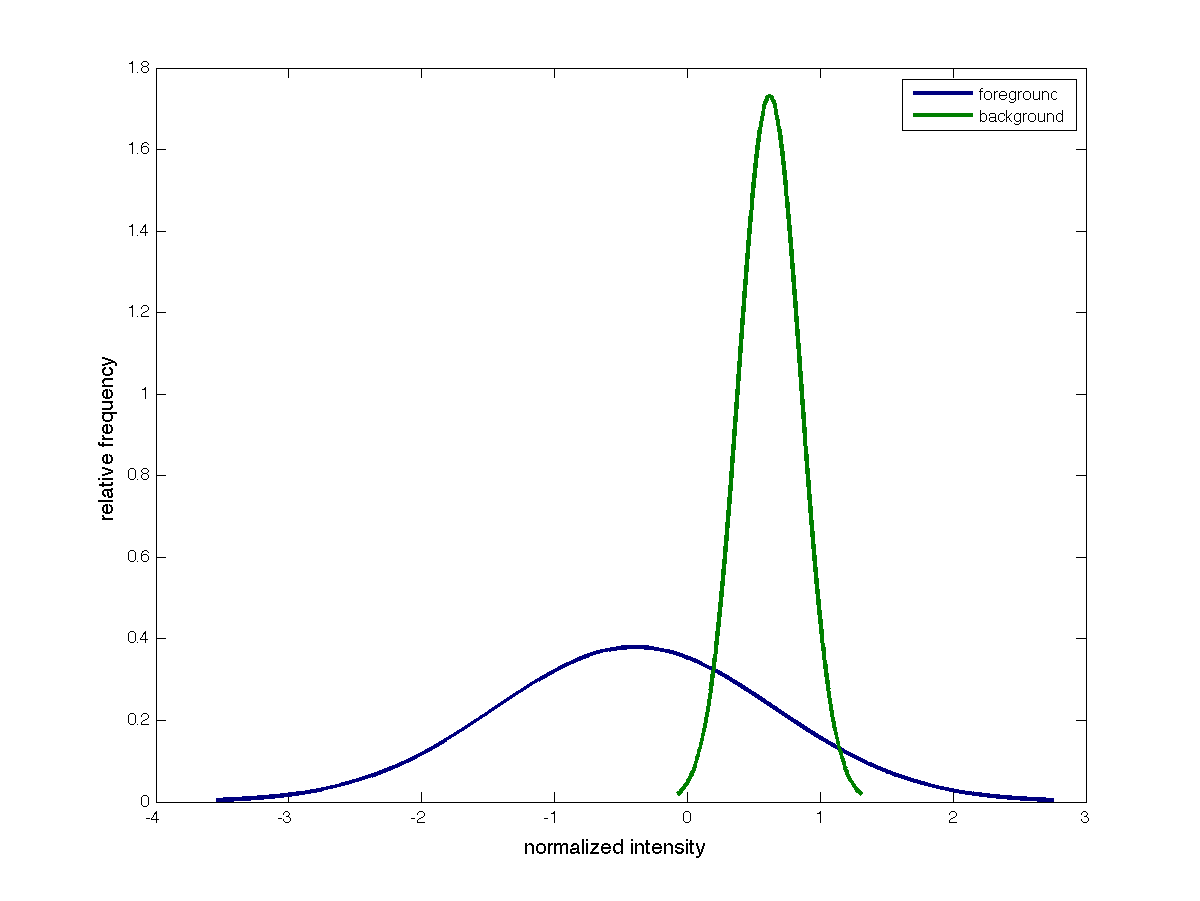
\includegraphics[width=\linewidth]{pics/distribution.png}
\caption{ Learned global foreground (in blue) $ p(x_{ij}\mid c=f,s_j)$ and
  background (in green) $p(x_{ij} \mid c=b,s_j)$ image intensity models }
\label{fig:distribution}
\end{figure}

\section{Learning the Emission Probabilities}
The annotated data $\truth$ does not contain segmentations of
vehicle-id characters from the background, rather the annotation are
loose bounding boxes that contain significant white-space. Thus,
\emph{Unsupervised learning} will be required to specify the
\emph{emissions probabilities} $p(x_{ij} \mid s_j)$.

Denote the set of parameters needed to determine the model of a glyph
column $j$ as
\[\model_{k_j}=\{\,\mu_1,\sigma_1,\mu_2,\sigma_2,\gamma_{1,k_j},\gamma_{2,k_j},\ldots,\gamma_{m,k_j}\,\}.\]
Then the model for all columns of all glyphs in the entire font set is
specified as
\[
\model = \cup_{i=1}^m\model_{k_i}.
\]

Given the annotated data $\truth$, we seek the maximum-likelihood
estimate \[ \optmodel = \argmax_{\model} \lhood(\truth \mid \model).\]

There was a significant variance of character width in the annotations
of \texttt{np-images-5000.mat}. This might be caused by annotation
errors or from image-rectification errors. To account for glyph-width
variance in the annotations during training, the median width for each
glyph was calculated, and the subset of exemplars from the training
set that matched the median width of a particular glyph were used to
build the model for that glyph's columns. Exemplars that differed from
teh median width were simply filtered out.

Learning a model for a glyph column comprises of learning the
position-independent global foreground $ p(x_{ij}\mid
c=f,s_j)=\mathcal{N}(x_{ij};\sigma_1,\mu_1)$ and background $p(x_{ij}
\mid c=b,s_j)=\mathcal{N}(x_{ij};\sigma_2,\mu_2)$ image intensity
models, as well their position-dependent and glyph-dependent
priors. The Expectation Maximization scheme is used to learn these
parameters.

\subsection{Estimating parameters by EM}
At the $t+1$ E-step, for each license plate $d$ in the annotated
dataset \truth, the probability of intensity $x^d_{ij}$ of license $d$
is calculated with respect to given model $\model^t$:
\[
  p^{t+1}(x^d_{ij} \mid c=f, s_j) =
  \frac{\mathcal{N}(x^d_{ij};\sigma_1^t,\mu_1^t)\gamma_{is_j}^t}{\mathcal{N}(x^d_{ij};\sigma_1^t,\mu_1^t)\gamma_{is_j}^t+\mathcal{N}(x^d_{ij};\sigma_2^t,\mu_2^t)(1-\gamma_{is_j}^t)}
\]

At the $i+1$ M-step, the model parameters $\model^{t+1}$ are
maximized with respect to $p^{t+1}(x \mid c=f, s)$:
\[
  \gamma_{is_j}^{t+1} = \frac{\sum_{d \in \mathcal{D}} p^{t+1}(x^d_{ij} \mid
    c=f, s_j)}{\sum_{d \in \mathcal{D}} p^{t+1}(x^d_{ij} \mid c=f,
    s_j) + \sum_{d \in \mathcal{D}} (1-p^{t+1}(x^d_{ij} \mid c=b,
    s_j))}
\]
\[
  \sigma_1^{t+1} = \frac{\sum_{i,j} \sum_{d \in \mathcal{D}} x^d_{
      ij} p^{t+1}(x^d_{ij} \mid c=f, s_j)}{\sum_{i,j} \sum_{d \in
      \mathcal{D}} p^{t+1}(x^d_{ij} \mid c=f, s_j)}
\]
The parameters $\sigma_2^{t+1}, \mu_1^{t+1}, \mu_2^{t+1}$ are
calculated analogously. Estimation alternates between E-step and
M-step until the stopping condition
$|1-\frac{\sigma_1^{t+1}}{\sigma_1^{t}}| < \epsilon \wedge
|1-\frac{\sigma_2^{t+1}}{\sigma_2^{t}}| < \epsilon$ holds, where
$\epsilon$ is set to $10^{-5}$.

\begin{figure}[htp]
\centering
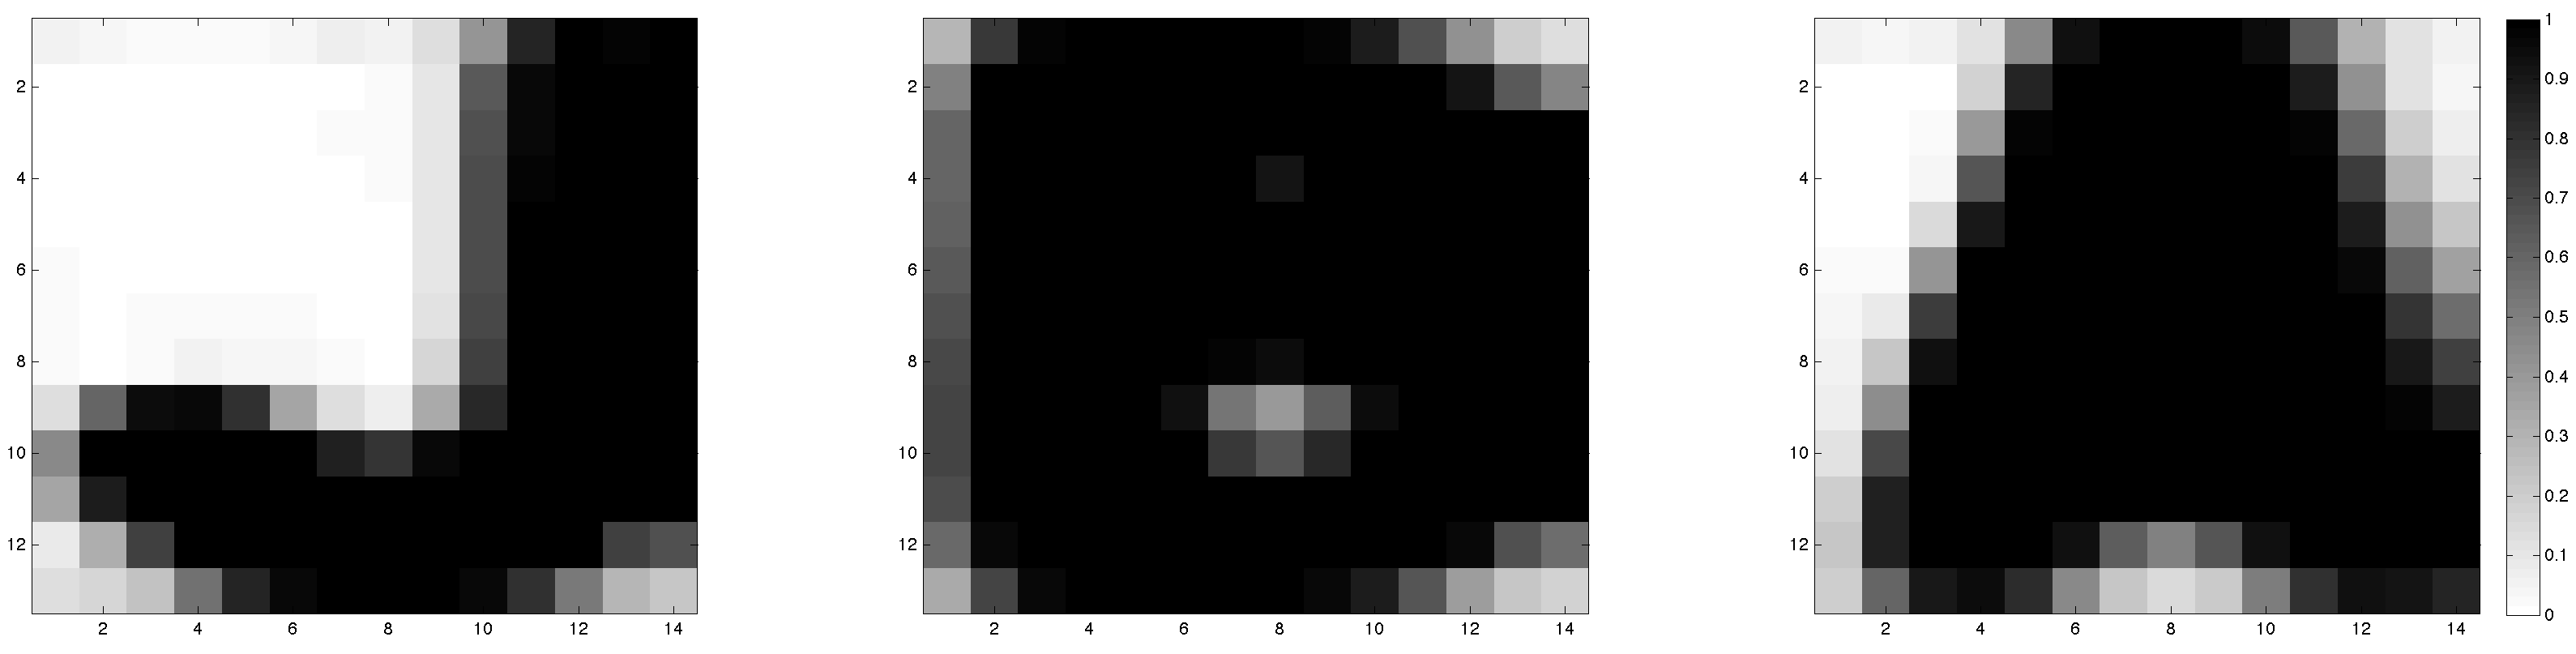
\includegraphics[width=\linewidth]{pics/jba.png}
\caption{Learned templates of \texttt{J}, \texttt{B} and
  \texttt{A}. Intensity corresponds to the prior probability for being
  a foreground pixel.}
\label{fig:templates}
\end{figure}

\section{Setting the Transition Probabilities}
Permitted transitions were set by hand based on some qualitative
observations of the given license-plate data. Allowed transitions
include white-space to white-space, white-space to first glyph
columns, between consecutive glyph columns, between terminal glyph
columns and white-space. Additionally, to allow for variance in
character widths, we allow transitions to the same glyph
column. Transitions to non-consecutive glyph columns and from
non-terminal glyph columns to white-space are prohibited.

Transition probabilities were also derived qualitatively from the
data. For example, the expected value of the length of white-space
intervals $E[W]$ was empirically estimated to be about $10$ from the
annotated data after image cropping, and the transition probability
from white-space to white-space was set as follows 
\[ 
E[W] = \sum_{k=1}^\infty k\,p(X=k) = \sum_{k=1}^\infty k
\,p(s_i=\text{w}y \,| s_{i-1})=\text{w})^k \implies p(s_i=\text{w} \,|
s_{i-1}) = 2-\sqrt{\frac{4}{E[W]}}.
\]

\section{Inference}
The hamming loss function is used for inference. As discussed above,
the HMM contains transitions with zero probabilities. For example, we
do not allow a transition from glyph column $A_5$ to white-space.
Care must be taken to avoid inferring invalid sequences of hidden
states.  Finding a valid sequence of hidden states that minimizes risk
under the hamming loss is equivalent to minimizing the expected
hamming loss over the subset of hidden states that have non-zero
transitions.  
To find the most probable valid sequence $s$, the probabilities
$p(x,s_i)$ are first computed by multiplying $p(x_1,\ldots,x_i,s_i)$
and $p(x_{i+1},\ldots,x_n|s_i)$, each of which can be computed
dynamically in $\mathcal{O}(|K|^2n)$. Selecting
$k^*=\argmax_k{p(x,s_i=k)}$ for each $i$ could give a sequence $s$
that is invalid.  This is computed dynamically with complexity
$\mathcal{O}(|K|n)$.

\begin{figure}[h]
  \centering
  \subfloat[correct id]{\label{fig:PBL2432}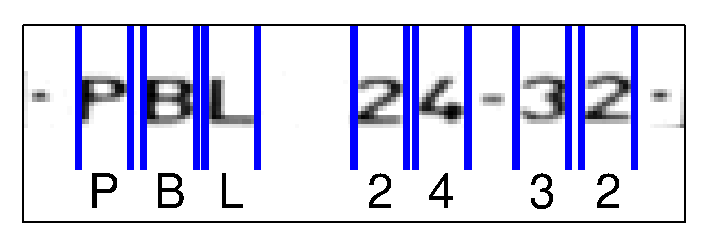
\includegraphics[width=0.3\textwidth]{matlab/lic_PBL2432.eps}}                
  \subfloat[\texttt{0} confused with \texttt{D}]{\label{fig:KLL72D8}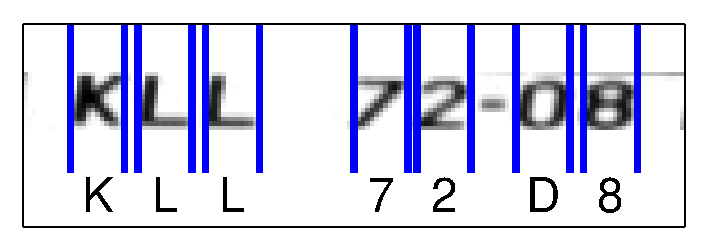
\includegraphics[width=0.3\textwidth]{matlab/lic_KLL72D8.eps}}
  \subfloat[\texttt{Z} confused with \texttt{2}]{\label{fig:mouse}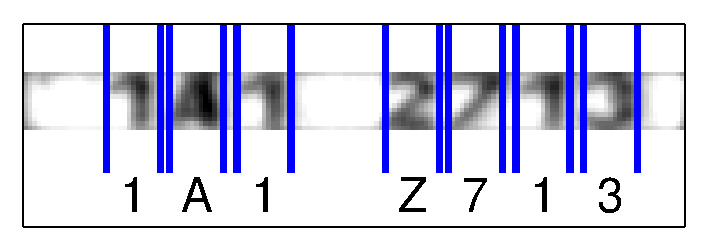
\includegraphics[width=0.3\textwidth]{matlab/lic_1A1Z713.eps}}
  \caption{Inferred vehicle ids from license plate images. Bottom
    line of text is the inferred string. Pairs of vertical blue bars
    are intervals of columns that were segmented as containing a
    character.}
  \label{fig:inferred-strings}
\end{figure}

\section{Evaluation}
Performance was measured on the test set \texttt{np-images-5000.mat}
consisting of 5000 annotated images of license plates.  Note that a
subset of the test set was used for training emissions distributions
too. Of interest is the quality of segmentation and the the accuracy of
license-id inference.

Correct segmentation of a character occurs when an interval of columns
inferred by the HMM as a character, called an \emph{inferred character
  region}, sufficiently overlaps an interval of columns annotated by
hand as a character, called an \emph{annotated character region}. A
correct segmentation of the license plate occurs when all annotated
characters regions are segmented correctly. Given license plate $k$ in
test set \test, an annotated white-space or character region $i$
of license plate $k$, denoted $R^k_i$, is said to be sufficiently
overlapped by an inferred character region of license plate $k$,
denoted $\hat{R^k_j}$, if

\[
\left|1-\frac{|R^k_i \cap \hat{R}^k_j|}{|R^k_i|}\right| < 0.15
\] 

The probability of detection $p_d$ is defined as the ratio of correct
segmentations to the total number of annotated character regions in
the test set. The probability of false alarm $p_{fa}$ is defined as
the number of annotated white-space regions that are inferred as
character regions by the HMM to the total number annotated white-space
regions. Results for \texttt{np-images-5000.mat} are given in Table
\ref{table:segmentation}.

\begin{table}[ht]
\begin{center}
\begin{tabular}{|l|l|}
  \hline
  \multicolumn{2}{|c|}{Segmentation Performance} \\
  \hline
  $p_d$ & 71.9\% \\
  $p_{fa}$ & 7.60\% \\
  \hline
\end{tabular}
\caption{Calculated for \texttt{np-images-5000.mat}}
\label{table:segmentation}
\end{center}
\end{table}

We require a metric on strings so that closeness of the inferred
vehicle-id to the annotated vehicle-id can be measured. The
Lenvenstein distance function $d_L$ between two strings is defined as
the minimum number of edits needed to transform one string into the
other, with the allowable edit operations being insertion, deletion,
or substitution of a single character.

\begin{figure}[ht]
\begin{center}
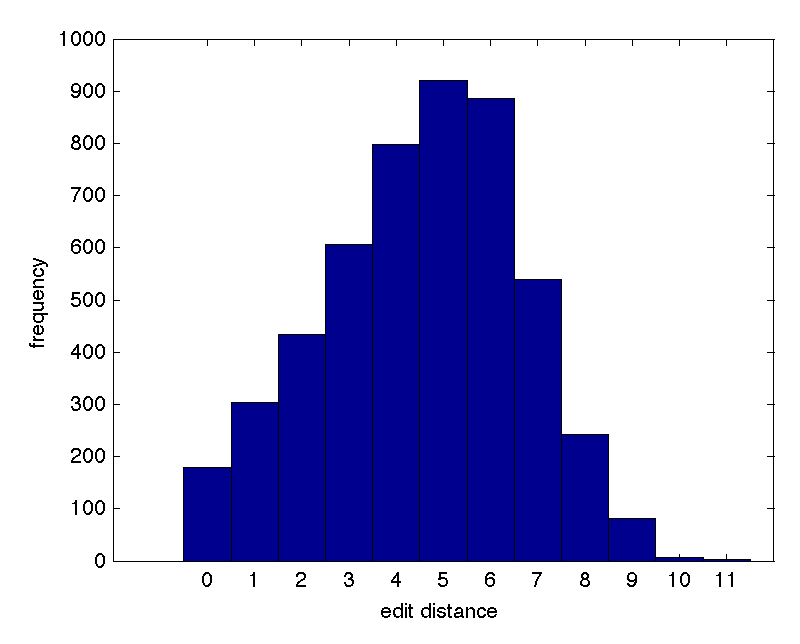
\includegraphics[width=0.75\linewidth]{matlab/hamming.eps}
\caption{ Frequency of edit distance over \texttt{np-images-5000.mat}  } 
\label{fig:editdistance}
\end{center}
\end{figure}

To determine the accuracy of the estimated vehicle-ids for the
\texttt{np-images-5000.mat} test set, the expected Levenstein distance
between inferred vehicle-id and annotated vehicle-id is computed for
all 5000 images.

\[ \text{accuracy} = \frac{\sum_{k \in \test}
  d_L(\hat{id}_k,id_k)}{7|\test|} \qquad \test \text{ is test set
  \texttt{np-images-5000.mat} }  \]

\begin{table}[ht]
\begin{center}
\begin{tabular}{|l|l|}
  \hline
  \multicolumn{2}{|c|}{ID accuracy} \\
  \hline
  $accuracy$ & 36.5\% \\
  \hline
\end{tabular}
\caption{Calculated for \texttt{np-images-5000.mat}}
\end{center}
\end{table}

\section{Analysis and Suggested Improvements}
The performance, as suggested by the evaluation above, is not suitable
for operational use. The HMM made many assumptions, some of which were
adopted to speed development; thus, there are many improvements to
consider for better performance. As expected, the HMM works best on
clean and typical exemplars from the test set.

There was a significant variance of character width in the annotations
of \texttt{np-images-5000.mat}. This might be caused by annotation
errors or from image-rectification errors. As previously discussed, to
account for glyph-width variance in the annotations during testing,
the median width for each glyph was calculated, and the subset of
exemplars from the test set that matched the median width of a
particular glyph were used to build the model for that glyph's
columns. Although expedient for development, throwing away problematic
annotations meant that our templates would not be representative of
some of the badly conditioned data. Inference was sure to suffer
because of this design choice. An improvement would be to normalize
the characters to a canonical coordinate system and learn mixture
parameters in this representation.

To account for varying character widths during inference, we allowed
for non-zero transitions to the same glyph column.  This allowance
enables the inference algorithm to cope with characters that are wider
than the template. Because of the difficulty in choosing appropriate
transition probabilities, we chose to prohibit non-zero transitions to
non-consecutive glyph columns. Easing this restriction would enable
the inference algorithm to robustly cope with characters narrower than
the template and would likely have a significant performance benefit.

The transition model does not account for cases where there is no
apparent white space between characters, which happens when there is
significant blur. Additionally, we did not create a template for
hyphens which occur in a significant number of the license
plates. Explicit modeling of the two aforementioned cases would likely
eliminate some of the more obvious segmentation errors.

Setting the transition probabilities manually was guided by some
simple observations from the training set. It is inevitable that we
missed some interactions in the data. Moving to supervised learning to
set the transition probabilities would likely capture relations in the
data that were overlooked.

Perhaps most problematic is the overlap and large variance of the
global intensity models (see Figure \ref{fig:distribution}) estimated
during training. Ideally, without de-focus blur and image artifacts,
since the license plate is a high contrast object, there should be two
well-separated intensity distributions, each with smaller variance. To
account for image corruption, more than two classes might be used to
classify intensities that are neither distinctly part of foreground
nor background.

Lastly, there was no explicit model created for the license plate
string. In other the words, prior information on the expected number
of characters, or the expected location of white space and hyphens was
not included. It is likely that these hard constraints would
dramatically improve performance. 
\end{document}
